\documentclass[conference]{IEEEtran}
\IEEEoverridecommandlockouts
% The preceding line is only needed to identify funding in the first footnote. If that is unneeded, please comment it out.
\usepackage{cite}
\usepackage{amsmath,amssymb,amsfonts}
\usepackage{graphicx}
\usepackage{textcomp}
\def\BibTeX{{\rm B\kern-.05em{\sc i\kern-.025em b}\kern-.08em
    T\kern-.1667em\lower.7ex\hbox{E}\kern-.125emX}}
\begin{document}

\title{THE2\\
}

\author{\IEEEauthorblockN{Esref Ozturk}
\IEEEauthorblockA{\textit{CENG} \\
\textit{METU}\\
Ankara, Turkey \\
esrefozturk93@gmail.com}
}

\maketitle


\section{Introduction}
This report includes the discussions about CENG499 Machine Learning THE2 Homework \\

\section{Discussion}

\subsection{Feature Scaling Technique}

Min-Max scaling technique is used for scaling each  features to 0-1 range. Using min-max scaling, all different range features are scaled to the same range. Luckily there was no feature that has the same max and min so min-max scaling were used.

\subsection{Effects of the Different Architectures}

I tried 5 different architectures:\\
\begin{itemize}
    \item No Hidden Layers
    \item 1 Hidden Layer with 1 Neuron
    \item 1 Hidden Layer with 3 Neurons
    \item 2 Hidden Layer with 3 Neurons
    \item 3 Hidden Layer with 3 Neurons
\end{itemize}

Their plots can be found on the Plots section. \\
For all architectures, error of set2 was dropping more rapidly at first but then set1 is converging quick. I  think that's related to structure of the data.\\
Adding more layers resulting in sudden drops at some points and overall coverging time got shorter.

\subsection{When to Stop Updates}

As it can be seen in the previous subsection, all lines are converging after some amount of epochs. We can stop updated there.


\subsection{Training and Validation Sets}

80\% of training set is used for training the models and 20\% is used for validation.


\section{Plots}

\subsection{No Hidden Layers: Set1 and Set2}

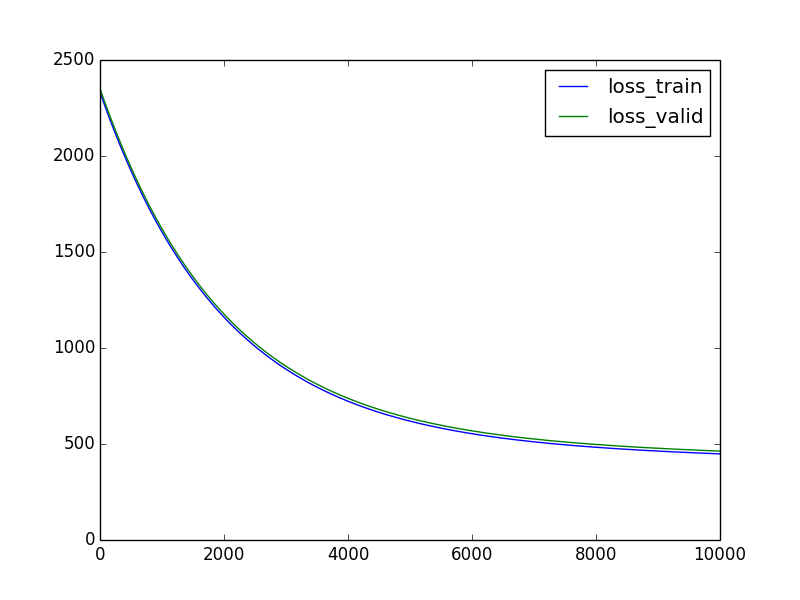
\includegraphics[width=0.5\textwidth]{set1-[].png}
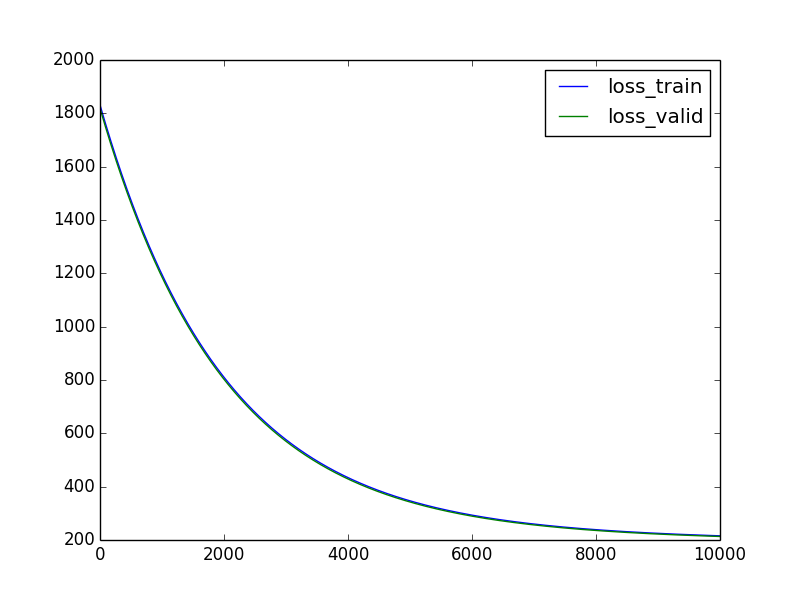
\includegraphics[width=0.5\textwidth]{set2-[].png}


\subsection{1 Hidden Layer with 1 Neuron: Set1 and Set2}

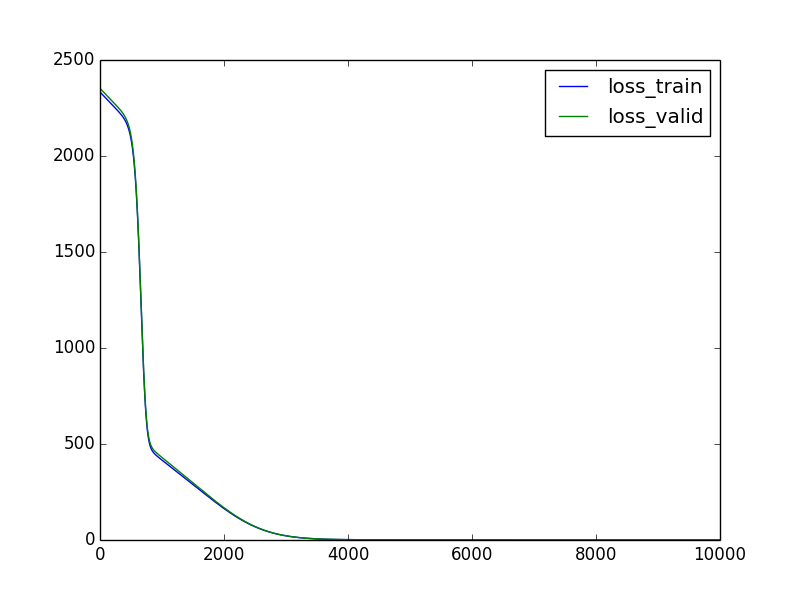
\includegraphics[width=0.5\textwidth]{set1-[1].png}
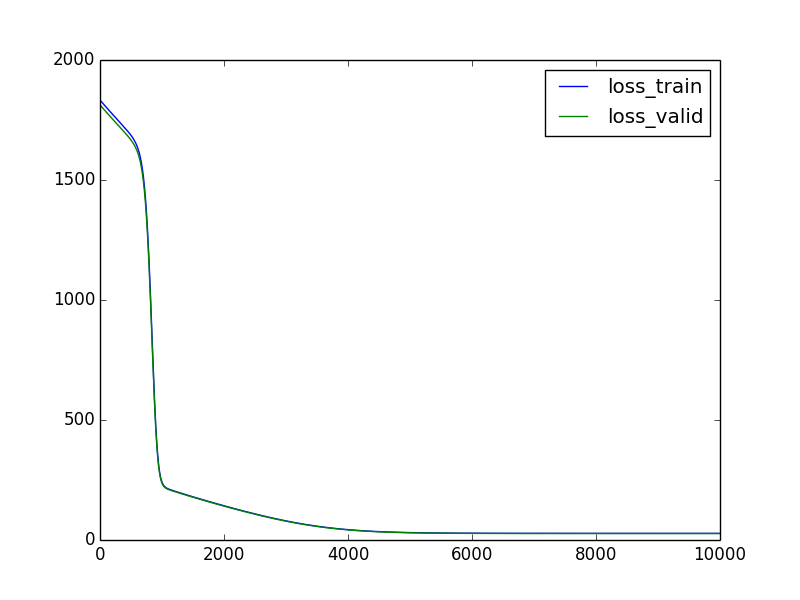
\includegraphics[width=0.5\textwidth]{set2-[1].png}


\subsection{1 Hidden Layer with 3 Neurons: Set1 and Set2}

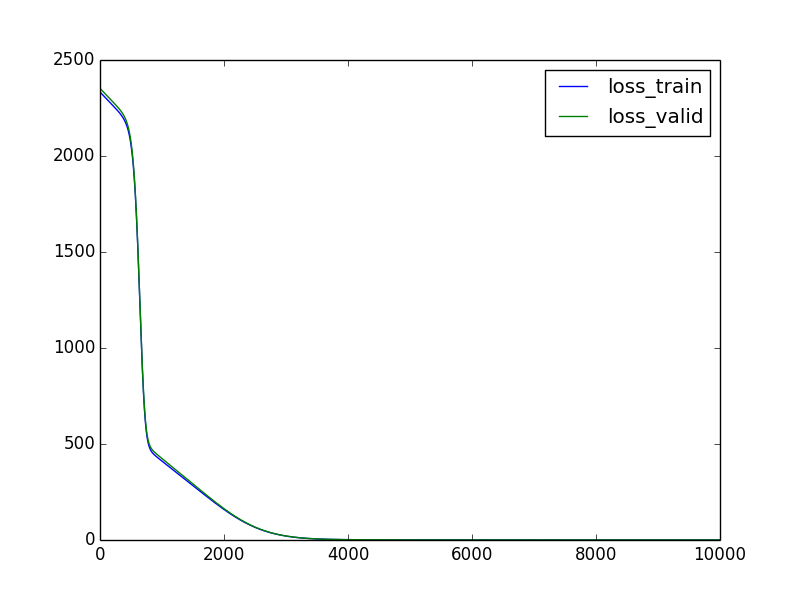
\includegraphics[width=0.5\textwidth]{set1-[3].png}
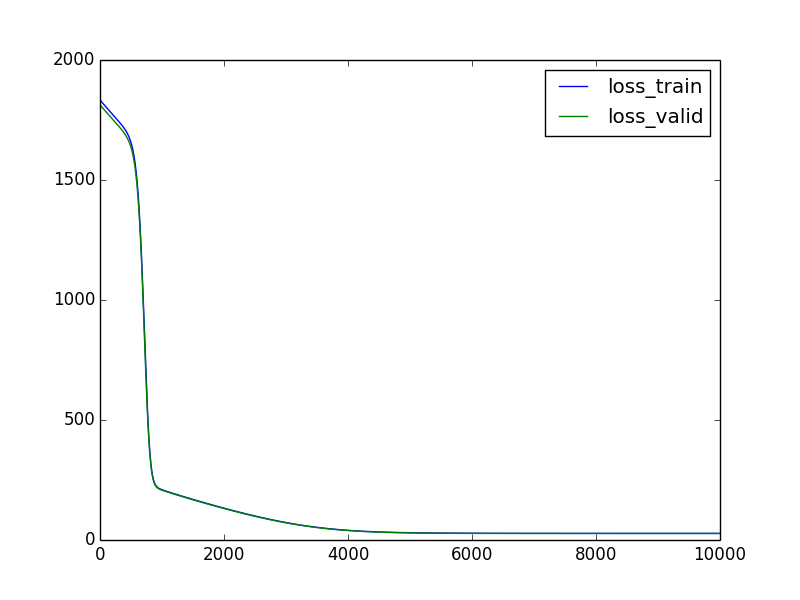
\includegraphics[width=0.5\textwidth]{set2-[3].png}

\subsection{2 Hidden Layer with 3 Neurons: Set1 and Set2}

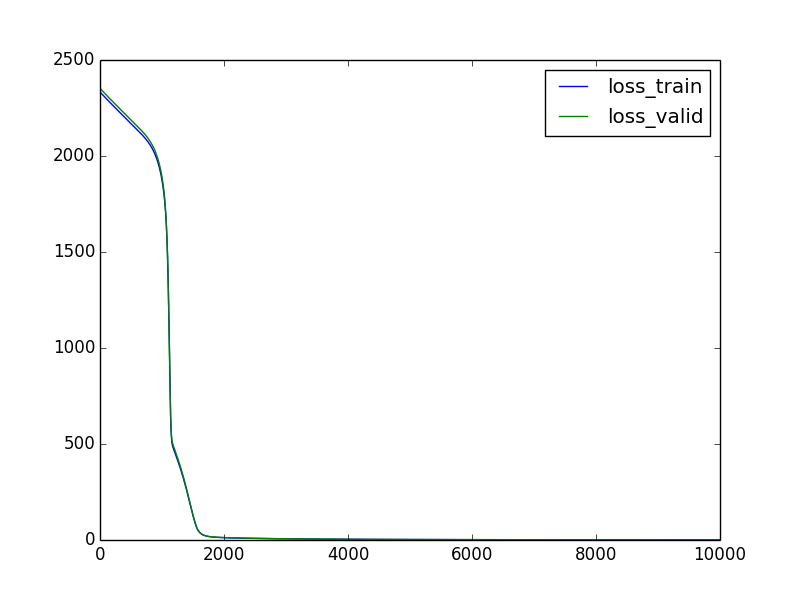
\includegraphics[width=0.5\textwidth]{set1-[3,3].png}
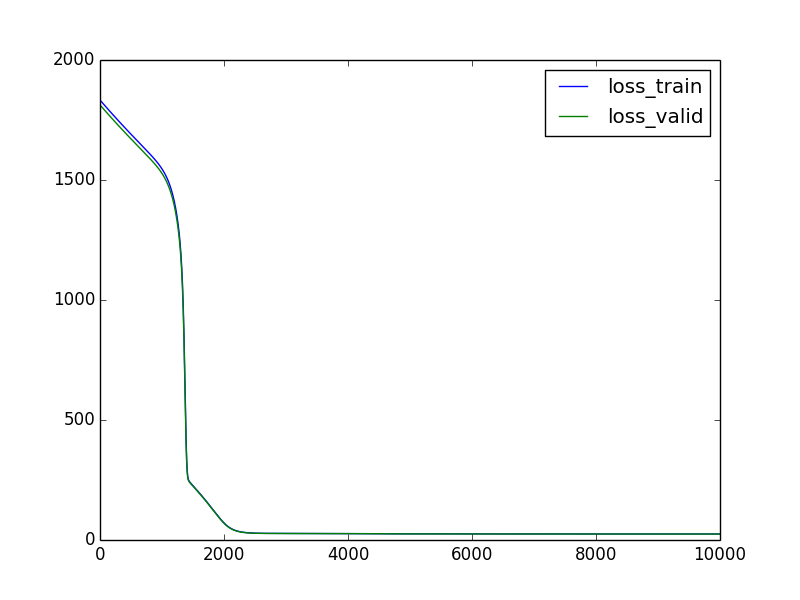
\includegraphics[width=0.5\textwidth]{set2-[3,3].png}

\subsection{3 Hidden Layer with 3 Neurons: Set1 and Set2}

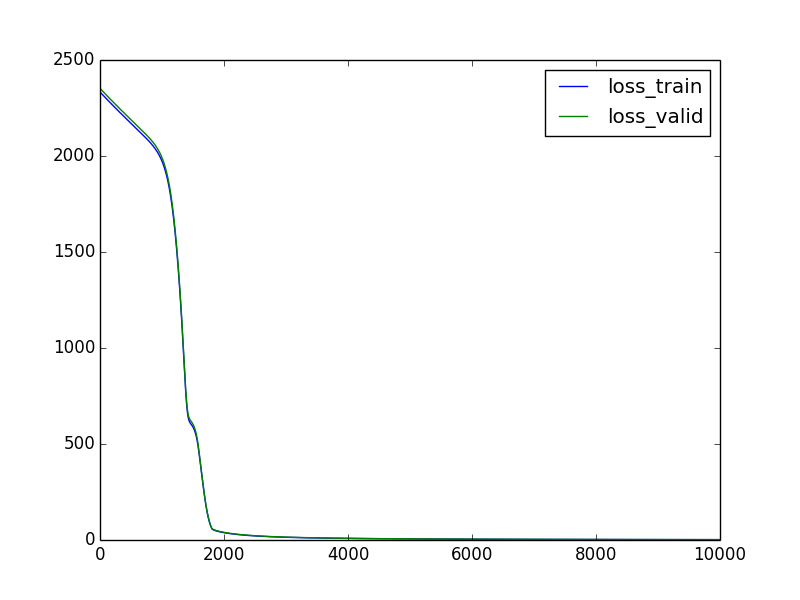
\includegraphics[width=0.5\textwidth]{set1-[3,3,3].png}
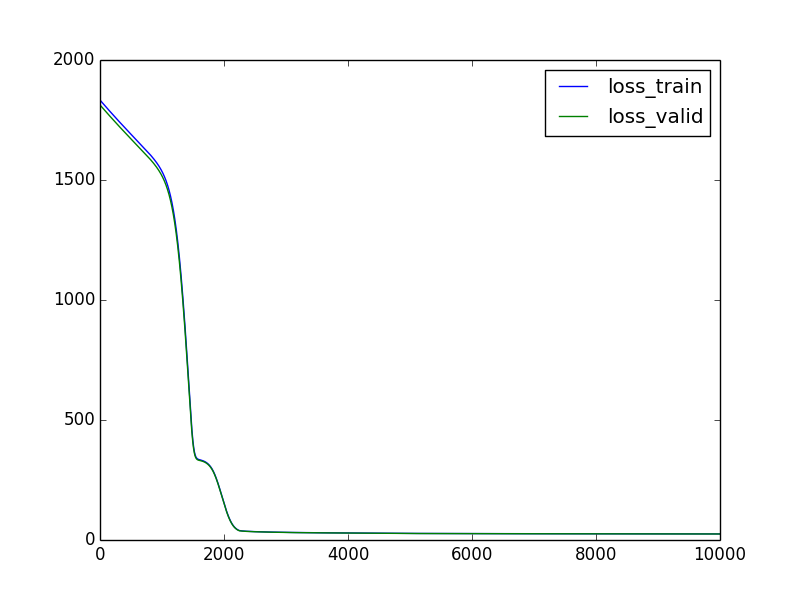
\includegraphics[width=0.5\textwidth]{set2-[3,3,3].png}



\section{Conclusion}
Using artificial neural networks for regression and analyzing error history is very cool idea.

\end{document}
